\documentclass[a4paper]{article}

\usepackage[english]{babel}
\usepackage{amsmath}
\usepackage{color}
\usepackage{amssymb}
\usepackage{dsfont}
\usepackage{multicol}
\usepackage[lofdepth,lotdepth]{subfig}
\usepackage{graphicx}
\usepackage{listings}
\usepackage[hyphens]{url}
\usepackage{pgf, tikz}
\usetikzlibrary{arrows, automata}
\usepackage{titling}
\usepackage{varwidth}
\usepackage{hyperref}
\usepackage{color} %red, green, blue, yellow, cyan, magenta, black, white
\definecolor{mygreen}{RGB}{28,172,0} % color values Red, Green, Blue
\definecolor{mylilas}{RGB}{170,55,241}
\setlength\parindent{0pt}
\usepackage{float}


\newcommand\independent{\protect\mathpalette{\protect\independenT}{\perp}}
\def\independenT#1#2{\mathrel{\rlap{$#1#2$}\mkern2mu{#1#2}}}

\usepackage{geometry}
 \geometry{
 a4paper,
 total={165mm,257mm},
 left=20mm,
 top=20mm,
 }

\definecolor{codegreen}{rgb}{0,0.6,0}
\definecolor{codegray}{rgb}{0.5,0.5,0.5}
\definecolor{codepurple}{rgb}{0.58,0,0.82}
\definecolor{backcolour}{rgb}{0.95,0.95,0.92}

\lstdefinestyle{mystyle}{
    backgroundcolor=\color{backcolour},   
    commentstyle=\color{codegreen},
    keywordstyle=\color{magenta},
    numberstyle=\tiny\color{codegray},
    stringstyle=\color{codepurple},
    basicstyle=\footnotesize,
    breakatwhitespace=false,         
    breaklines=true,                 
    captionpos=b,                    
    keepspaces=true,                 
    numbers=left,                    
    numbersep=5pt,                  
    showspaces=false,                
    showstringspaces=false,
    showtabs=false,                  
    tabsize=2
}
 
\lstset{style=mystyle}


\title{Statistical Machine Learning 2018\\Assignment 2\\Deadline: 28th of October 2018}
\author{
  Christoph Schmidl\\ s4226887\\      \texttt{c.schmidl@student.ru.nl}
  \and
  Mark Beijer\\ s4354834\\     \texttt{mbeijer@science.ru.nl}
}
\date{\today}

\begin{document}
\maketitle


\section*{Exercise 1 - weight 3}

The financial services department of an insurance company receives numerous phone calls each day from people who want to make a claim against their policy. Most claims are genuine, however about 1 out of every 6 are thought to be fraudulent. To tackle this problem the company has installed a trial version of a software voice-analysis system that monitors each conversation and gives a numerical score $z$ between 0 and 1, depending on allegedly suspicious vocal intonations of the customer. Unfortunately, nobody seems to know anymore how to interpret the score in this particular version of the system...\\

Tests revelealed that the conditional probability density of $z$, given that a claim was valid $(c = 1)$ or false $c = 0$ are 

\begin{align*}
p(z | c = 0) \quad &= \quad \alpha_o(1 - z^2),\\
p(z | c = 1) \quad &= \quad \alpha_1z(z + 1).
\end{align*}



\subsection*{1.1}

Compute the normalization constants $\alpha_0$ and $\alpha_1$. How does the $z$ score relate to the validity of the claim? What values for $z$ would you expect when the claim is valid / false?\\

\textbf{Answer:}\\



\subsection*{1.2}

Use the sum and product rule to show that the probability distribution function $p(z)$ can be written as 

\begin{equation}
	p(z) = \frac{(3z + 1)(z + 1)}{4}
\end{equation}


\textbf{Answer:}\\




\subsection*{1.3}

Use Bayes' rule to compute the posterior probability distribution function $p(c|z)$. Plot these distributions in MATLAB as a function of $z$. How can these posterior probabilities help in making a decision regarding the validity of the claim?\\


\textbf{Answer:}\\



\subsection*{1.4}

Compute the optimal decision boundary (based on our numerical score $z$) that minimizes the misclassification rate. For which $z$ should we classify $c = 0$ (false) and for which $z$ should we classify $c = 1$ (valid)? Explain your decision.\\


\textbf{Answer:}\\



\subsection*{1.5}

Compute the misclassification rate, given the optimal decision boundary determined previously. Interpret the result you have obtained. Is the $z$ score useful in determining the validity of the claim? Compare this with your prior guess from 1.\\


\textbf{Answer:}\\




\section*{Exercise 2 - weight 2}

The government of the United Kingdom has decided to call a referendum regarding the country's European Union membership. The citizens of the UK will be asked the following question at the referendum: "Whould the United Kingdom remain a member of the European Union or leave the European Union?". The European Commission (EC) is interested in the potential outcome of this referendum and has contracted a polling agency to study this issue.\\
Suppose that a person's vote follows a Bernoulli distribution with paramter $\theta$ and suppose the the EC's prior distribution for $\theta$, the proportion of British citizens that would be in favor of leaving the EU, is beta distribution with $\alpha = 90$ and $\beta = 110$.


\subsection*{2.1}

Determine the mean and variance of the prior distribution. Plot the prior density function.\\

\textbf{Answer:}\\


The beta distribution is defined as:


\begin{equation}
Beta(\mu|\alpha, \beta) = \frac{\Gamma (\alpha + \beta )}{\Gamma(\alpha) \Gamma(\beta)} \mu^{\alpha - 1}(1-\mu)^{\beta - 1}
\end{equation}


*Not sure if this is needed, but we can do it some time regardless.*************************\\
The mean is calculated as following:

\begin{eqnarray}
\mathbb E[\mu] &=& \int_0^{1} \text{Beta(}\mu|\alpha,\beta) \mu d \mu \\
&=& \int_0^1 \frac{\Gamma (\alpha + \beta )}{\Gamma(\alpha) \Gamma(\beta)} \mu^{\alpha}(1-\mu)^{\beta - 1} d\mu \\
&=& \frac{\Gamma (\alpha + \beta )}{\Gamma(\alpha) \Gamma(\beta)} \int_0^1 \mu^{\alpha}(1-\mu)^{\beta - 1} d\mu 
\end{eqnarray}

**************************************************
%Bishop page 71
The mean and variance are therefore:

\begin{eqnarray}
\mathbb E [\mu] &=& \frac{\alpha}{\alpha + \beta } = 4.5\cdot 10^{-1}\\
 var [\mu ] &=& \frac{\alpha \beta}{(\alpha + \beta)^2(\alpha + \beta + 1)} \approx 1.23 \cdot 10^{-3}
\end{eqnarray}

\begin{figure}[H]
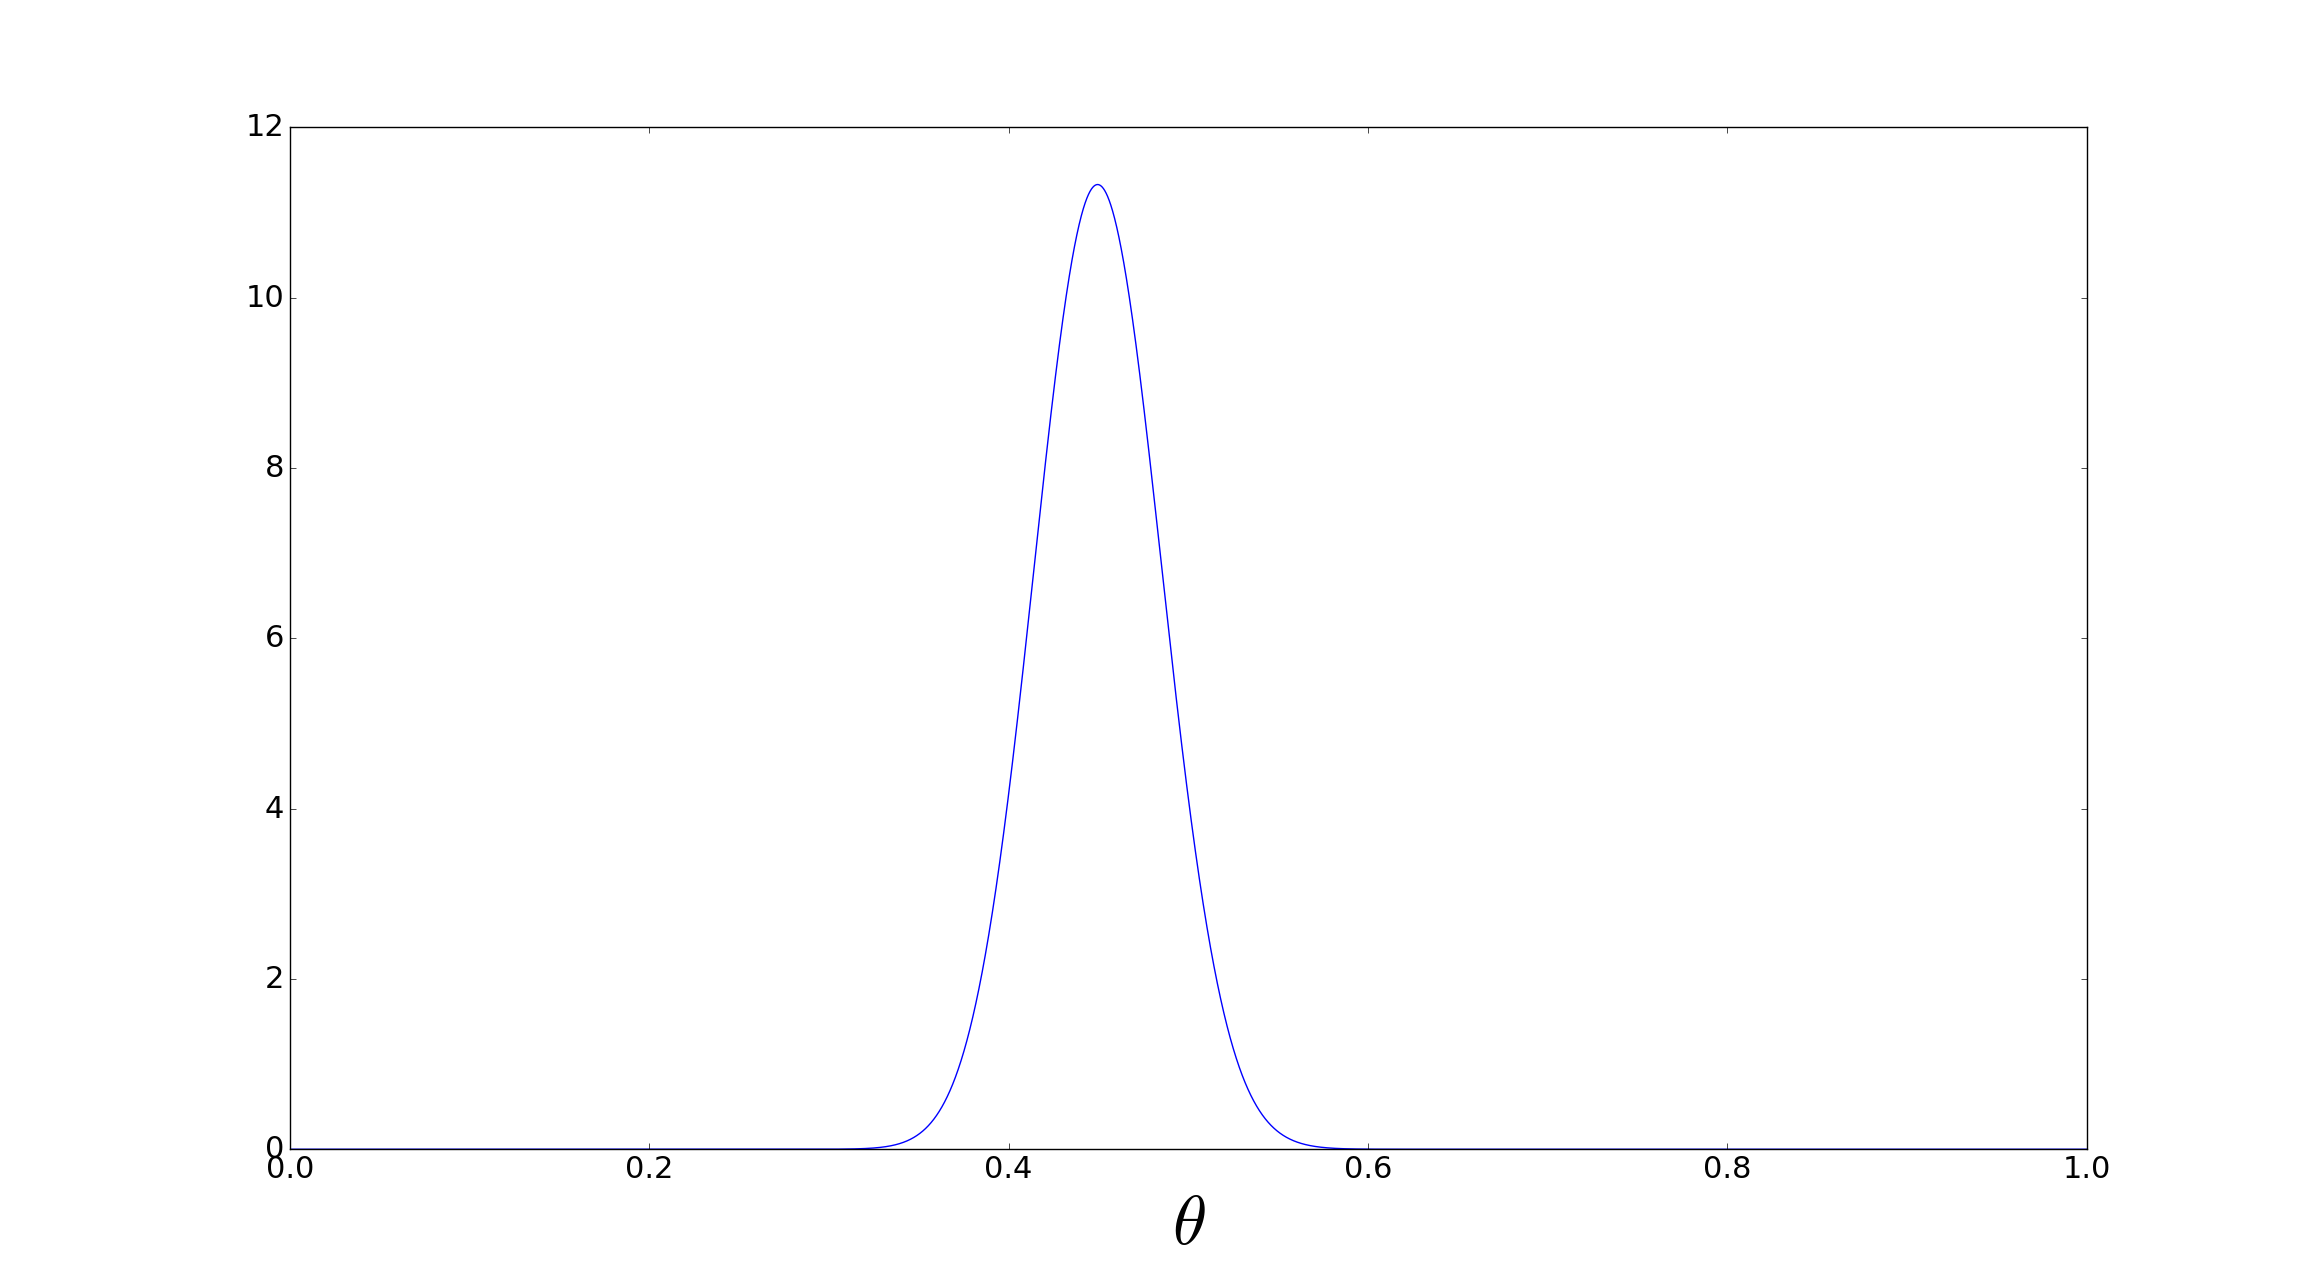
\includegraphics[width=\textwidth]{BetaPlotEx2.png}
\caption{Plot of the beta distrubition for $alpha$ = 90 and $\beta$ = 110.}
\end{figure}





\subsection*{2.2}

A random sample of 1000 British citizens is taken, and 60\% of the people polled support leaving the European Union. What are the posterior mean and variance for $\theta$? Plot the posterior density function together with the prior density. Explain how the data from the sample changed the prior belief.\\

\textbf{Answer:}\\

The posterior probabilty is described as:

\begin{equation}
p(\mu|m,l,\alpha,\beta) = \frac{\Gamma(m+\alpha+l+\beta)}{\Gamma(m+\alpha)\Gamma(l+\beta)} \mu^{m+\alpha-1}(1-\mu)^{l+\beta-1}
\end{equation}

So the value of $\alpha$ is increased by m and the value of $\beta$ is increased by l.The value of m is the amount of people in support, the value of m is how many people will vote in favour, while l is how many people will vote against. So the new mean is:

\begin{eqnarray}
\mathbb E [\mu] &=& \frac{\alpha + m}{\alpha + m + \beta + l}= 5.75 \cdot 10^{-1}\\
var[\mu]  &=& \frac{(\alpha + m ) ( \beta + l)}{(\alpha + \beta + l + m)^2(\alpha + \beta + m + l + 1 )} = 2.03\cdot 10^{-4}
\end{eqnarray}




\subsection*{2.3}

Examine the effect of changing the prior hyperparameters $(\alpha, \beta)$ on the posterior by looking at several other hyperparamter configurations. Which values for $\alpha$ and $\beta$ correspond to a non-informative prior? What is the interpretation of $\alpha$ and $\beta$ for the beta prior? What does the choice of $\alpha$ and $\beta$ in Question 1 tell you about the strength of the prior belief?\\


\textbf{Answer:}\\






\subsection*{2.4}

Imagine you are now a reporter for the polling agency and you have been sent on field duty to gather more data. Your mission is to go out on the streets and randomly survey people on their thoughts regarding the upcoming referendum. Given all the available information you have acquired, what is the probability that the first person you talk to will vote 'Leave'?\\

\textbf{Hint:} Derive the predictive distribution for the next vote using the posterior distribution for $\theta$ computed in Question 2. For a reminder on predictive distribution, see subsection 1.2.6 in Bishop, in particular Equation (1.68).\\


\textbf{Answer:}\\





\section*{Exercise 3 - Sequential learning (weight 5)}


\textbf{Part 1 - Obtaining the prior}

Consider a four dimenstional variable $[x_1, x_2, x_3, x_4]^T$, distributed according to a multivariate Gaussian with mean $\tilde{\mu} = [1,0,1,2]^T$ and covariance matrix $\tilde{\Sigma}$ given as

	
\[ \tilde{\Sigma} = 
	\left(
	\begin{array}{cc|cc}
	0.14 & -0.3 & 0.0 & 0.2 \\
	-0.3 & 1.16 & 0.2 & -0.8 \\
	\hline
	0.0 & 0.2 & 1.0 & 1.0 \\
	0.2 & -0.8 & 1.0 & 2.0 \\	
	\end{array}
	\right)
\]	

We are interested in the conditional distribution over $[x_1,x_2]^T$, given that $x_3 = x_4 = 0$. We know this conditional distribution will also take the form of a Gaussian:

\begin{equation}
p([x_1,x_2]^T \; | \; x_3 = x_4 = 0) = \mathcal{N}([x_1,x_2]^T \; | \; \mu_p, \Sigma_p) \label{eq:part1}
\end{equation}

for which the mean and covariance matrix are most easily expressed in terms of the (partitioned) precision matrix (see Bishop, §2.3.1).



\subsection*{3.1.1}

Use the partitioned precision matrix $\tilde{\Lambda} = \tilde{\Sigma}^{-1}$ to give an explicit expression for the mean $\mu_p$ and covariance matrix $\Sigma_p$ of this distribution and calculate their values. (This distribution will be taken as the prior information for the rest of this exercise, hence the subscript p). You may use the MATLAB command \texttt{inv} to calculate the matrix inverses.\\

\textbf{Answer:}\\



\subsection*{3.1.2}

[MATLAB] - Create a function that can generate random number pairs, distributed according to the distribution in \ref{eq:part1}. Initialize your random generator and the draw a single pair

\begin{equation}
	\mu_t = [\mu_{t1}, \mu_{t2}]^T
\end{equation}

from this distribution. (These will be the 'true' means, hence the subscript t).\\

\textbf{Hint:} you can use the MATLAB function \texttt{mvnrnd} (which resides the Statistics toolbox).\\

\textbf{Answer:}\\




\subsection*{3.1.3}

[MATLAB] - Make a plot of the probability density of the distribution \ref{eq:part1}.\\

\textbf{Hint:} Use the MATLAB function \texttt{mvnpdf} (which resides in the Statistics toolbox) to calculate the probability density of a multivariate Gaussian random variable. The MATLAB functions \texttt{meshgrid} and \texttt{surf} may also prove useful.\\


\textbf{Answer:}\\

\textbf{Part 2 - Generating the data}

Here we assume we are dealing with a 2d-Gaussian daa generating process

\begin{equation}
	p(x) = \mathcal{N}(x|\mu, \Sigma)
\end{equation}

For the mean $\mu$, we will use the value $\mu_t$ drawn in \ref{} in order to generate the data. Subsequently, we will pretend that we do not know this "true" value $\mu_t$ of $\mu$, and estimate $\mu$ from the data. For the covariance matrix $\Sigma$ we will use the "true" value

\[ \Sigma_t = \left( \begin{array}{cc}
2.0 & 0.8  \\
0.8 & 4.0 \end{array} \right)\] 

to generate the data.


\subsection*{3.2.1}

[MATLAB] - Generate at least 1000 data pairs $\{ x_i, y_i\}$, distributed according to \ref{} with $\mu = \mu_t$ and $\Sigma = \Sigma_t$ and save them to a file in plain-text format.\\

\textbf{Answer:}\\



\subsection*{3.2.2}

From now on, we will assume (pretend) the 'true' mean $\mu_t$ is unknown and estimate $\mu$ from the data. Calculate the maximum likelihood estimate of $\mu_{ML}$ and $\Sigma_{ML}$ for the data, and also an unbiased estimate of $\Sigma$ (see Bishop, §2.3.4). Compare with the true values $\mu_t$ and $\Sigma_t$.\\

\textbf{Answer:}\\



\textbf{Part 3 - Sequential learning algorithms}

We will now estimate the mean $\mu$ from the generated data and the known variance $\Sigma_t$ sequentially, i.e., by considering the data points one-by-one.

\subsection*{3.3.1}

[MATLAB] - Write a procedure that processes the data points $\{ x_n \}$ in the generated file one-by-one, and after each step comptues an updated estimate of $\mu_{ML}$, the maximum likelihood of the mean (using Bishop, eq. 2.126).\\


\textbf{Answer:}\\





\subsection*{3.3.2}


Now we also use the prior information $p(\mu) = \mathcal{N}(\mu | \mu_p, \Sigma_p)$. From the prior, the generated data and the known variance $\Sigma_t$, we will estimate the mean $\mu$.\\

Work out the details of sequential Bayesian inference (see eq. 2.144) for the mean $\mu$. Apply Bayes' theorem in eq. 2.113 - 2.117 at each step $n = 1, ..., N$ to compute the new posterior mean $\mu^{(n)}$ and covariance $\Sigma^{(n)}$ after a new point $(x_n)$ has arrived from the old posterior step. The first step starts from the original prior \ref{}.\\
\textbf{Note:} Do not confuse the posterior $\Sigma^{(n)}$ with the known $\Sigma_t$ of the data generating process. For some more hints, see appendix.\\

\textbf{Answer:}\\


\subsection*{3.3.3}

[MATLAB] - Write a procedure that processes the data points $\{ x_n\}$ in the generated file one-by-one, and after each step computes an updated estimate of $\mu_{MAP}$ - the maximum of the posterior distribution, using the results of the previous exercise.\\


\textbf{Answer:}\\


\subsection*{3.3.4}

[MATLAB] - Plot both estimates (ML and MAP) in a single graph (1d or 2d) as a function of the number of data points observed. Indicate the true values $\{ \mu_{t1}, \mu_{t2}\}$ as well. Evaluate your result.\\

\textbf{Answer:}\\

\section*{Hints}

Below are some hints for \textbf{Exercise 3 - Part 3 - Question 2}.\\

Bayes'r rule is also valid if earlier acquired information is taken into account. For example, if this is earlier seen data $D_{n - 1} = \{ x_1,..., x_{n - 1}\}$. Bayes' rule conditioned on this earlier data is 

\begin{align*}
	P(\mu | x_n, D_{n - 1}) \propto P(\mu | D_{n - 1}) P(x_n | \mu, D_{n - 1})
\end{align*}

Since $D_n = \{ x_1, ..., x_n\}$ this is written more conveniently as 

\begin{align*}
	P(\mu | D_{n}) \propto P(\mu | D_{n - 1}) P(x_n | \mu, D_{n - 1})
\end{align*}


If, given the model paramters $\mu$, the probability distribution of $x_n$ is independent of earlier data $D_{n - 1}$, we can further reduce this to

\begin{align*}
	P(\mu | D_{n}) \propto P(\mu | D_{n - 1}) P(x_n | \mu)
\end{align*}

You should be able to see the realtion with (2.144) and see in particular that the factor between brackets in (2.144) is to be identified with $P(\mu | D_{n - 1})$.\\
Another important insight is that if $P(\mu | D_{n - 1})$ and $P(x_n | \mu)$ are of the form (2.113) and (2.114), i.e., if $P(\mu | D_{n - 1})$ is a Gaussian distribution over $\mu$ with a certain mean and covariance (you are free to give these any name, e.g. $\mu^{(n-1)}, \Sigma^{(n-1)}$) and if $P(x_n | \mu)$ is also Gaussian with a mean that is linear $\mu$, then you can use (2.116) and (2.117) to compute the posterior $P(\mu | D_n)$, which therefore is also Gaussian.\\
So it is your task to show this. To do this you have to figure out the mapping of the variables and parameters in the current exercise, i.e., what is the correspondence between $\mu, x_n, \Sigma_t, \mu^{(n-1)}, \Sigma^{(n-1)}$ etc. with $x, \mu, \Lambda, A, b, L$. Don't forget that some quantities can also be zero or and other may be identity matrices.



\end{document}
